\chapter{Analysis and specification of requirements}
\minitoc
\newpage

\setcounter{secnumdepth}{0} % Set the section counter to 0 so next section is not counted in toc
% ----------------------- Introduction ----------------------- %
\section{Introduction}
In this chapter, I analyze the various specifications and requirements of modernizing Navoy's AI travel platform from development to production.
I describe the platform's main features, microservices architecture requirements, and the DevSecOps practices that must be implemented for the end result.

\setcounter{secnumdepth}{2} % Resume counting the sections for the toc with a depth of 2 (Sections and sub-sections)
% ----------------------------------- SECTIONS (v) ----------------------------------- %
% ----------------------- Functional Requirements ----------------------- %
\section{Functional requirements}
The modernization of Navoy's AI travel platform requires implementing several core functionalities across multiple microservices based on the defined system architecture:

\subsection{REST Gateway Service}
\begin{itemize}
    \item \textbf{API Management:} Serve as the public-facing entry point for all API users with centralized access control.
    \item \textbf{Rate Limiting \& Caching:} Implement Redis-based rate limiting and caching mechanisms for optimal performance.
    \item \textbf{Access Management:} Integrate SaaS and API customer flows efficiently with comprehensive authentication.
    \item \textbf{API Documentation:} Provide comprehensive REST endpoint documentation for external developers.
\end{itemize}

\subsection{User Service}
\begin{itemize}
    \item \textbf{Authentication \& Authorization:} Manage secure user login, role verification, and multi-factor authentication.
    \item \textbf{User Profile Management:} Handle user profiles, organizations, and role-based access control (RBAC).
    \item \textbf{Multi-tenancy Support:} Enable both B2C and B2B user management with organizational hierarchies.
    \item \textbf{Session Management:} Maintain secure user sessions with OAuth 2.0 integration.
\end{itemize}

\subsection{Trip Generator Service}
\begin{itemize}
    \item \textbf{AI-Driven Trip Creation:} Generate personalized travel itineraries using generative AI based on user preferences.
    \item \textbf{Asynchronous Processing:} Handle trip generation requests via RabbitMQ for improved scalability.
    \item \textbf{Data Integration:} Fetch travel data from internal services and external APIs for comprehensive recommendations.
    \item \textbf{Itinerary Storage:} Store generated trips in MongoDB with flexible document structures.
\end{itemize}

\subsection{Travel Data Sync Service}
\begin{itemize}
    \item \textbf{External API Synchronization:} Sync travel data from external providers (Viator, Amadeus) into local MongoDB.
    \item \textbf{Scheduled Data Updates:} Run cron jobs to ensure fresh and consistent travel data availability.
    \item \textbf{Performance Optimization:} Maintain local dataset for quick access by trip-generator-service.
    \item \textbf{Data Consistency:} Handle API change notifications and maintain data integrity across services.
\end{itemize}

\subsection{Viator Adapter Service}
\begin{itemize}
    \item \textbf{API Adaptation:} Provide RESTful interface to Viator API with simplified integration for clients.
    \item \textbf{Product Information Access:} Enable trip-generator to access relevant travel product information.
    \item \textbf{Data Compatibility:} Ensure seamless integration with synchronized MongoDB database.
    \item \textbf{Client Access:} Support both API users and SaaS platform through REST gateway.
\end{itemize}

\subsection{Billing Service}
\begin{itemize}
    \item \textbf{Subscription Management:} Handle subscription plans and pay-per-use billing for B2C and B2B clients.
    \item \textbf{Usage Tracking:} Monitor API usage, quotas, and overages with real-time reporting.
    \item \textbf{Payment Integration:} Integrate with Stripe for secure payment processing and billing operations.
    \item \textbf{Billing Analytics:} Provide comprehensive billing reports and usage analytics.
\end{itemize}

\subsection{Vector Store Service}
\begin{itemize}
    \item \textbf{Embedding Generation:} Create vector store embeddings through RabbitMQ consumer integration.
    \item \textbf{gRPC Interface:} Provide queried embeddings via gRPC connect service for efficient data retrieval.
    \item \textbf{ChromaDB Integration:} Interface with ChromaDB vector database for semantic search capabilities.
    \item \textbf{AI Enhancement:} Support advanced AI features with vector-based similarity matching.
\end{itemize}

\subsection{Content Management Service}
\begin{itemize}
    \item \textbf{Content Management:} Manage static pages, blogs, travel information, and media assets.
    \item \textbf{Non-technical User Interface:} Provide user-friendly CMS interface for content updates.
    \item \textbf{Media Asset Management:} Handle storage and organization of travel-related media content.
    \item \textbf{PostgreSQL Integration:} Store structured content with efficient database management.
\end{itemize}

\subsection{Platform Web Application}
\begin{itemize}
    \item \textbf{SaaS Frontend:} Provide modern, responsive web interface for end-users.
    \item \textbf{Trip Management:} Enable users to generate, modify, and manage travel itineraries.
    \item \textbf{User Account Management:} Handle user preferences, bookings, and account settings.
    \item \textbf{API Integration:} Interface with all backend services through REST gateway.
\end{itemize}

\subsection{Travel Platform Dashboard}

\subsubsection*{\underline{Use case}}
\begin{figure}[H]
    \centering
    \makebox[\textwidth]{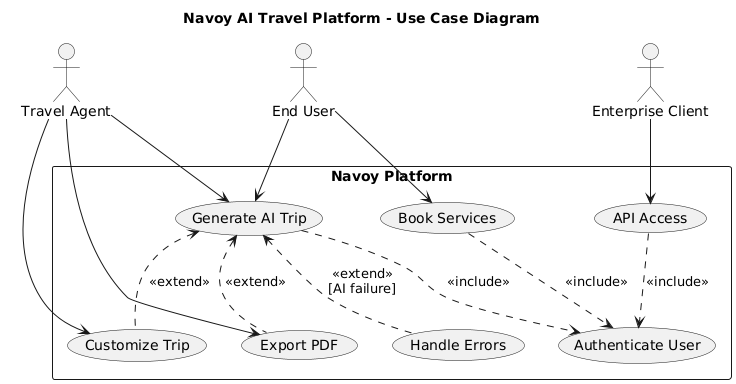
\includegraphics[width=\linewidth]{src/assets/diagrams/usecase.png}}
    \caption{Use case diagram for Navoy's AI travel platform}
    \label{fig:use-case-diagram}
\end{figure}

\subsubsection{\underline{Use case textual description}}
Here is an example of the textual description of one of the key use case scenarios:
\begin{table}[H]
    \renewcommand{\arraystretch}{1.5}%
    \caption{Generate AI Trip Itinerary use case textual description}
    \centering
    \medskip
    \begin{tabularx}{1\textwidth} {
            | >{\hsize=0.5\hsize\linewidth=\hsize\centering\arraybackslash}X
            | >{\hsize=1.5\hsize\linewidth=\hsize\justifying\arraybackslash}X |}
        \hline
        \textbf {Use Case}         & \noindent Generate AI Trip Itinerary                                                                                                                                                            \\
        \hline
        \textbf {Actor}            & \noindent Travel Agent or End User.                                                                                                                                                             \\
        \hline
        \textbf {Pre-condition}    & \noindent Authenticated User with valid session.                                                                                                                                                \\
        \hline
        \textbf {Post-condition}   & \noindent Personalized trip itinerary generated and saved.                                                                                                                                      \\
        \hline
        \textbf {Basic path}       & \noindent    \begin{enumerate}
            \item Navigate to trip planning page.
            \item Enter travel preferences (destination, dates, budget, interests).
            \item Select travel style and accommodation preferences.
            \item Click "Generate AI Itinerary" button.
            \item Review generated itinerary with AI recommendations.
            \item Save or modify the generated trip plan.
        \end{enumerate}                                                                                                                                                         \\
        \hline
        \textbf {Exceptional path} & \noindent If AI service is unavailable, display fallback message and offer manual trip planning options. If user preferences are incomplete, prompt for required information before proceeding. \\
        \hline
    \end{tabularx}
\end{table}

% ----------------------- Conception ----------------------- %
\section{System Architecture and Technical Design}
In this section, I present the detailed architecture conception for Navoy's AI travel platform, including the microservices design, data flows, and technical infrastructure.

\subsection{Overall System Architecture}
The platform follows a microservices architecture pattern with eight core services, each responsible for specific business capabilities. The architecture emphasizes modularity, scalability, and maintainability while supporting both B2C SaaS users and B2B API clients.

\begin{figure}[H]
    \centering
    \makebox[\textwidth]{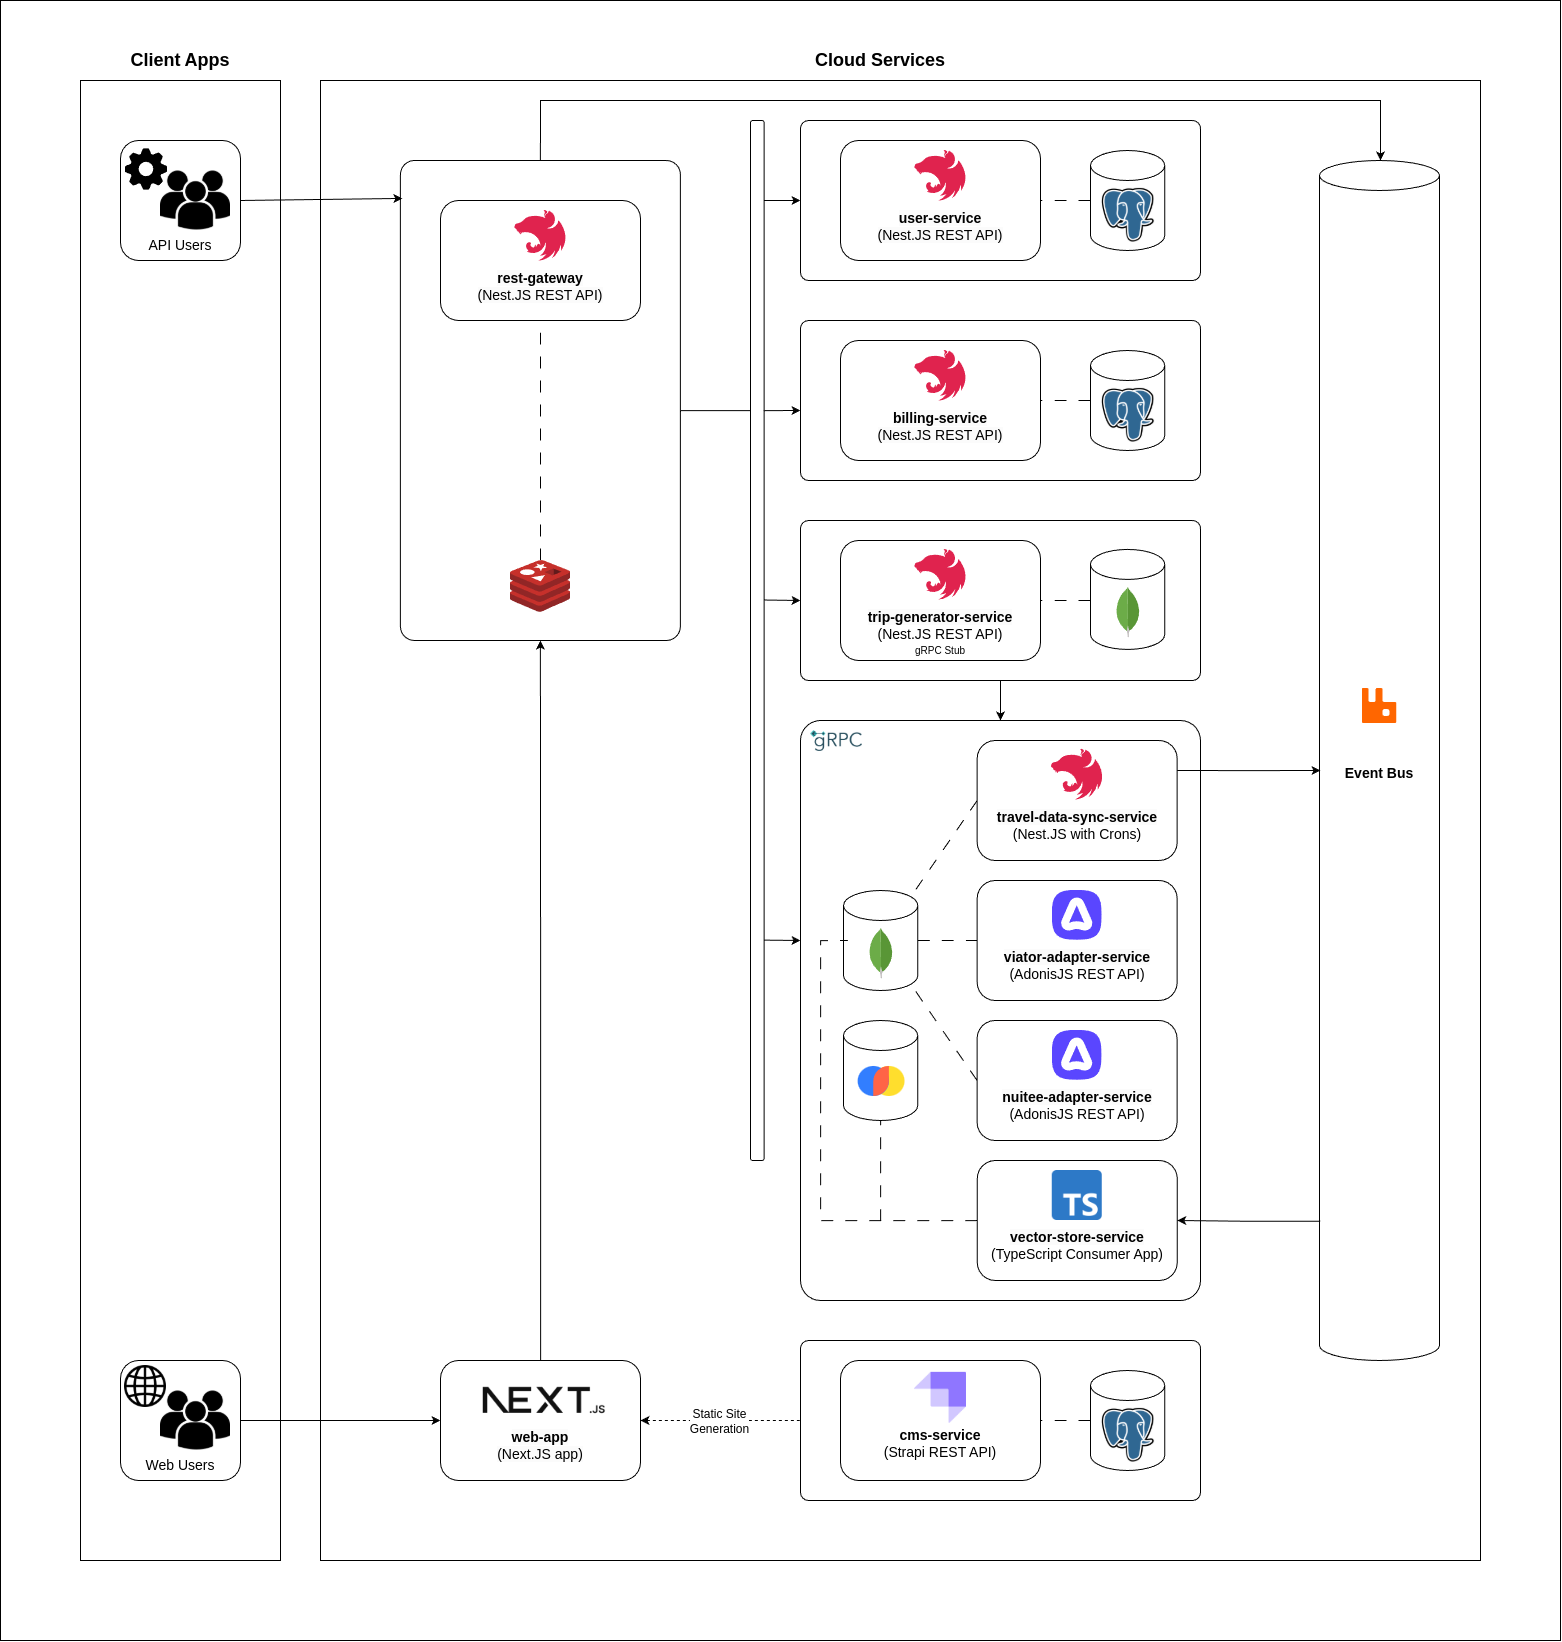
\includegraphics[width=0.9\linewidth]{./src/assets/diagrams/software-architecture.drawio.png}}
    \caption{Navoy AI Travel Platform - System Architecture Overview}
    \label{fig:system-architecture}
\end{figure}

\subsection{Core Microservices Design}

\subsubsection*{\underline{REST Gateway Service}}
\textbf{Technology Stack:} Node.js with Express, Redis for caching and rate limiting\\
\textbf{Primary Functions:}
\begin{itemize}
    \item Centralized API entry point for all external requests
    \item Redis-based rate limiting and response caching
    \item Request routing to appropriate backend services
    \item Authentication token validation and authorization
    \item Comprehensive API documentation with OpenAPI specifications
\end{itemize}

\subsubsection*{\underline{User Service}}
\textbf{Technology Stack:} Node.js, PostgreSQL, JWT authentication\\
\textbf{Primary Functions:}
\begin{itemize}
    \item Multi-tenant user authentication and authorization
    \item Role-based access control (RBAC) for organizations
    \item User profile and preference management
    \item OAuth 2.0 integration with third-party providers
    \item Session management with secure token handling
\end{itemize}

\subsubsection*{\underline{Trip Generator Service}}
\textbf{Technology Stack:} Python, FastAPI, MongoDB, RabbitMQ, LiteLLM\\
\textbf{Primary Functions:}
\begin{itemize}
    \item AI-powered trip itinerary generation using GPT and Claude models
    \item Asynchronous trip processing through RabbitMQ messaging
    \item Integration with travel data sources for comprehensive recommendations
    \item Flexible MongoDB schema for storing complex trip structures
    \item Real-time status updates for trip generation progress
\end{itemize}

\subsubsection*{\underline{Travel Data Sync Service}}
\textbf{Technology Stack:} Python, MongoDB, Celery for task scheduling\\
\textbf{Primary Functions:}
\begin{itemize}
    \item Automated synchronization with external travel APIs (Viator, Amadeus)
    \item Scheduled data updates using cron-based task scheduling
    \item Data transformation and normalization for consistent internal format
    \item Change detection and incremental update mechanisms
    \item Performance optimization through local data caching
\end{itemize}

\subsection{Data Architecture and Storage Strategy}

\subsubsection*{\underline{Database Design Pattern}}
The platform implements a "database per service" pattern to ensure service autonomy and data ownership:

\begin{table}[H]
    \renewcommand{\arraystretch}{1.3}
    \caption{Service Database Allocation}
    \centering
    \medskip
    \begin{tabularx}{1\textwidth} {
            | >{\hsize=0.6\hsize\linewidth=\hsize\centering\arraybackslash}X
            | >{\hsize=0.7\hsize\linewidth=\hsize\centering\arraybackslash}X
            | >{\hsize=0.7\hsize\linewidth=\hsize\justifying\arraybackslash}X |}
        \hline
        \textbf{Service} & \textbf{Database} & \textbf{Data Types}                          \\
        \hline
        User Service     & PostgreSQL        & User profiles, organizations, roles          \\
        \hline
        Trip Generator   & MongoDB           & Trip documents, itineraries, preferences     \\
        \hline
        Travel Data Sync & MongoDB           & Synchronized travel data, external API cache \\
        \hline
        Billing Service  & PostgreSQL        & Subscriptions, invoices, usage metrics       \\
        \hline
        CMS Service      & PostgreSQL        & Content pages, media metadata                \\
        \hline
        Vector Store     & ChromaDB          & Embeddings, semantic search indices          \\
        \hline
        Gateway          & Redis             & Rate limiting, session cache, API metrics    \\
        \hline
    \end{tabularx}
\end{table}

\subsubsection*{\underline{Inter-Service Communication Patterns}}

\textbf{Synchronous Communication:}
\begin{itemize}
    \item REST APIs for real-time operations requiring immediate responses
    \item gRPC for high-performance internal service communication (Vector Store)
    \item HTTP/HTTPS with JSON payloads for external API integrations
\end{itemize}

\textbf{Asynchronous Communication:}
\begin{itemize}
    \item RabbitMQ for trip generation requests and processing workflows
    \item Event-driven architecture for data synchronization notifications
    \item Message queues for decoupled service interactions
\end{itemize}

\subsection{AI and Machine Learning Integration}

\subsubsection*{\underline{LLM Integration Architecture}}
The platform integrates multiple AI providers through a unified interface:

\begin{itemize}
    \item \textbf{LiteLLM Proxy:} Unified interface for OpenAI GPT, Anthropic Claude, and other LLM providers
    \item \textbf{Model Selection:} Dynamic model routing based on request complexity and cost optimization
    \item \textbf{Prompt Engineering:} Specialized prompts for travel itinerary generation and recommendations
    \item \textbf{Response Processing:} Structured output parsing and validation for consistent trip data
\end{itemize}

\subsubsection*{\underline{Vector Store and Semantic Search}}
\begin{itemize}
    \item \textbf{ChromaDB Integration:} Vector database for storing travel destination and activity embeddings
    \item \textbf{Embedding Generation:} Automated embedding creation for travel content through RabbitMQ workers
    \item \textbf{Similarity Search:} Semantic matching for personalized travel recommendations
    \item \textbf{gRPC Interface:} High-performance querying for real-time similarity searches
\end{itemize}

\subsection{External API Integration Strategy}

\subsubsection*{\underline{Travel Service Providers}}
\begin{itemize}
    \item \textbf{Viator API:} Tours and activities booking through dedicated adapter service
    \item \textbf{Amadeus API:} Flight and hotel data synchronization
    \item \textbf{Travel Partner APIs:} Extensible adapter pattern for future integrations
\end{itemize}

\subsubsection*{\underline{Payment and Billing}}
\begin{itemize}
    \item \textbf{Stripe Integration:} Secure payment processing for subscription and pay-per-use billing
    \item \textbf{Usage Tracking:} Real-time API quota monitoring and billing calculation
    \item \textbf{Multi-tier Pricing:} Support for different subscription levels and enterprise contracts
\end{itemize}

% --------------- Non functional Requirements --------------- %
\section{Non-functional requirements}
Non-functional requirements describe specifications that do not add direct business value but are crucial for the reliable operation of the AI travel platform.
For Navoy's modernized platform, I focus on DevSecOps practices, performance optimization, and operational excellence.

\subsection{Performance and Scalability Requirements}
\begin{itemize}
    \item \textbf{Response Time:} AI trip generation must complete within 10-15 seconds for complex multi-destination itineraries
    \item \textbf{API Throughput:} Support 1000+ concurrent API requests with sub-200ms response times for standard queries
    \item \textbf{Auto-scaling:} Kubernetes HPA (Horizontal Pod Autoscaler) based on CPU/memory usage and custom metrics
    \item \textbf{Database Performance:} MongoDB queries optimized for <100ms response time with proper indexing strategies
    \item \textbf{Caching Strategy:} Redis-based caching with 95\% cache hit ratio for frequently accessed travel data
\end{itemize}

\subsection{Reliability and Availability Requirements}
\begin{itemize}
    \item \textbf{High Availability:} 99.9\% uptime SLA with multi-zone deployment across AWS regions
    \item \textbf{Fault Tolerance:} Circuit breaker patterns for external API dependencies with graceful degradation
    \item \textbf{Data Backup:} Automated daily backups with point-in-time recovery capabilities for all databases
    \item \textbf{Disaster Recovery:} RTO (Recovery Time Objective) of 4 hours and RPO (Recovery Point Objective) of 1 hour
    \item \textbf{Health Monitoring:} Comprehensive health checks, liveness/readiness probes for all microservices
\end{itemize}

\subsection{Security and Compliance Requirements}
\begin{itemize}
    \item \textbf{Authentication Security:} Multi-factor authentication, OAuth 2.0, and JWT token management with rotation
    \item \textbf{Data Encryption:} TLS 1.3 for data in transit, AES-256 encryption for sensitive data at rest
    \item \textbf{API Security:} Rate limiting (1000 req/hour per API key), input validation, SQL injection prevention
    \item \textbf{Network Security:} VPC isolation, security groups, and WAF (Web Application Firewall) protection
    \item \textbf{Compliance:} GDPR compliance for EU users, PCI DSS for payment processing, SOC 2 Type II certification
\end{itemize}

\subsection{DevSecOps and Infrastructure Requirements}
\begin{itemize}
    \item \textbf{CI/CD Pipeline:} Fully automated GitOps workflows with GitHub Actions for build, test, and deployment
    \item \textbf{Security Scanning:} Integrated SAST/DAST security scans, container vulnerability scanning with Trivy
    \item \textbf{Infrastructure as Code:} Terraform for AWS infrastructure provisioning and Kubernetes manifests
    \item \textbf{Secret Management:} AWS Secrets Manager integration for secure credential and API key rotation
    \item \textbf{Code Quality Gates:} Minimum 80\% test coverage, ESLint/Pylint for code quality, SonarQube analysis
\end{itemize}

\subsection{Monitoring and Observability Requirements}
\begin{itemize}
    \item \textbf{Application Monitoring:} Prometheus and Grafana for metrics collection and visualization
    \item \textbf{Distributed Tracing:} Jaeger for request tracing across microservices with performance analysis
    \item \textbf{Centralized Logging:} ELK Stack (Elasticsearch, Logstash, Kibana) for log aggregation and search
    \item \textbf{Alerting:} PagerDuty integration for critical alerts with escalation policies
    \item \textbf{Business Metrics:} Custom dashboards for API usage, trip generation success rates, and user engagement
\end{itemize}

\subsection{Development and Maintenance Requirements}
\begin{itemize}
    \item \textbf{Documentation Standards:} OpenAPI specs for all REST APIs, architecture decision records (ADRs)
    \item \textbf{Testing Strategy:} Unit tests (80\% coverage), integration tests, E2E tests with Playwright
    \item \textbf{Code Standards:} Consistent coding standards with automated formatting (Prettier, Black)
    \item \textbf{Deployment Strategy:} Blue-green deployments with canary releases for zero-downtime updates
    \item \textbf{Development Environment:} Docker Compose for local development, consistent dev-prod parity
\end{itemize}

\subsection{User Experience}
\begin{itemize}
    \item \textbf{Mobile Responsiveness:} Optimized experience across all device types and screen sizes.
    \item \textbf{Internationalization:} Multi-language support and currency conversion for global users.
    \item \textbf{Accessibility:} WCAG 2.1 compliance for inclusive user experience.
    \item \textbf{Offline Capability:} PDF export and limited offline functionality for trip access.
\end{itemize}
% ----------------------------------- SECTIONS (^) ----------------------------------- %

\setcounter{secnumdepth}{0} % Set the section counter to 0 so next section is not counted in toc
% ----------------------- Conclusion ----------------------- %
\section{Conclusion}
In this chapter, I conducted a comprehensive analysis of the requirements and architectural specifications for modernizing Navoy's AI travel platform.

I detailed the functional requirements across eight core microservices, each designed to handle specific business capabilities while maintaining service autonomy and scalability. The architecture leverages modern technologies including AI integration through LiteLLM, asynchronous processing with RabbitMQ, and vector-based semantic search with ChromaDB.

The technical design emphasizes a "database per service" pattern, ensuring data ownership and independence across microservices. I specified the integration patterns for both synchronous REST APIs and asynchronous message-driven communication, supporting the platform's dual nature as both a B2C SaaS application and B2B API service.

The non-functional requirements focus heavily on DevSecOps practices, establishing clear performance benchmarks (99.9\% uptime, sub-200ms API responses), comprehensive security measures (TLS 1.3, multi-factor authentication), and robust observability through monitoring, logging, and distributed tracing.

This architectural foundation provides the blueprint for implementing a scalable, secure, and maintainable AI travel platform that can handle enterprise-grade workloads while delivering exceptional user experiences. In the following chapter, I will detail the implementation and deployment strategies for realizing this technical vision.
